\documentclass[19pt]{beamer}
\usepackage{graphicx}
\usepackage{mdframed}

\setbeamertemplate{footline}[frame number]

\begin{document}

% \maketitle

% ................................................
\begin{frame}
\frametitle{Introduction}

Imagine driving in the dark, alert but not noticing a deer crossing the road right in front of you. Using stereo vision methods to see what is close, your car could detect the deer and brake before you even notice the obstacle. \\[10pt]
%
Stereo cameras could find distances, and sensing something closer than 20 feet, send the location to a computer controlling the car. The computer could reason that driving into the obstacle would be catastrophic and turn on the brakes. \\[10pt]
%
The deer, and you, would be safe.
\end{frame}
% ................................................


% ................................................
\begin{frame}
\frametitle{What is stereo matching?}

Stereo matching is a computer technique where two images taken from aligned cameras several centimetres apart are processed for depth information. \\[10pt]
%
For example, taking two images and using a simple algorithm, a colored image is returned, with blue color pixels closer than red color pixels. Here is an example, generated with my code.\\[20pt]

\centering
\setlength\tabcolsep{0.005\textwidth}
\begin{tabular}{ccc}
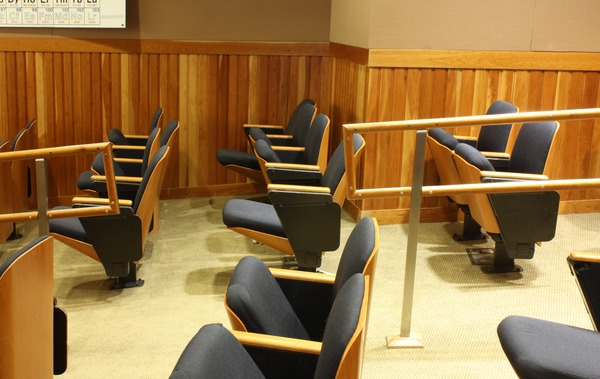
\includegraphics[width=0.33\textwidth]{images/im0-600.jpg} &
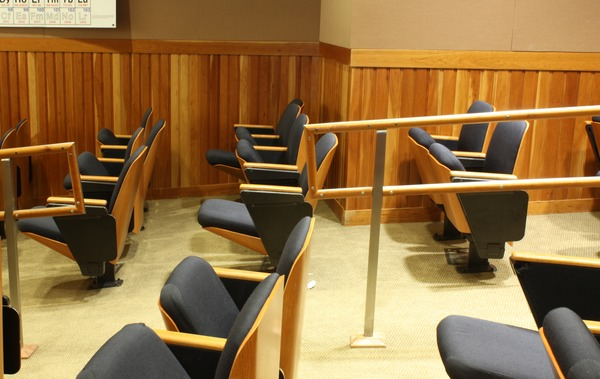
\includegraphics[width=0.33\textwidth]{images/im1-600.jpg} &
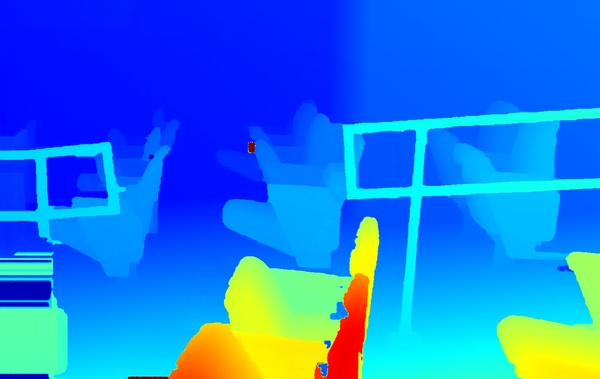
\includegraphics[width=0.33\textwidth]{images/disp-600.jpg} \\[2pt]
Left image & Right Image & Stereo matching \\
\end{tabular}

\end{frame}
% ................................................


% ................................................
\begin{frame}
\frametitle{Program Details}
\begin{enumerate}
    \item Calibrate stereo webcams\\[10pt]
    \item Capture images from stereo webcams\\[10pt]
    \item Find distances between images\\[10pt]
    \item Apply edge preserving median filter\\[10pt]
    \item Return the final disparity map 
\end{enumerate}
\end{frame}
% ................................................


% ................................................
\begin{frame}
\frametitle{Workflow 1: Calibrate stereo webcams}

When taking pictures for stereo vision, you need to make sure that the cameras are aligned exactly vertically and horizontally. If they aren't, the disparity map is noisy.\\[10pt]
%
To calibrate two cameras, you print a picture of a chessboard, and using an algorithm called SIFT key point detection, find the corners of the chessboard in both photos.\\[10pt]
%
Once you have the corners as key points, you can find the transformation matrix that maps from the left image to the right image. This will allow perfectly centering the cameras, resulting in  disparity maps with less noise.
\end{frame}
% ................................................


% ................................................
\begin{frame}
\frametitle{Workflow 2: Capture images from stereo webcams (1)}

My setup is a wooden board with 2 Microsoft LifeCam 3000 webcams mounted 2 centimeters apart, facing the same direction. \\[10pt]
%
This configuration can capture images of anything farther than three feet away, and works indoors and outdoors. This is a photograph of my webcam setup.\\

\begin{center}
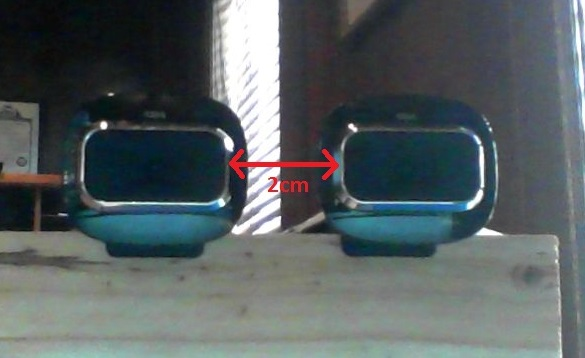
\includegraphics[width=0.75\textwidth, trim=30 50 45 50, clip]{images/setup.jpg}
\end{center}

\end{frame}
% ................................................


% ................................................
\begin{frame}
\frametitle{Workflow 2: Capture images from stereo webcams (2)}

The figure below shows two images of me in captured from the left and right webcams.\\[10pt]
%
This is a picture of me, from about 10 feet away.\\[20pt]

\begin{center}
\setlength\tabcolsep{0.01\textwidth}
\begin{tabular}{cc}
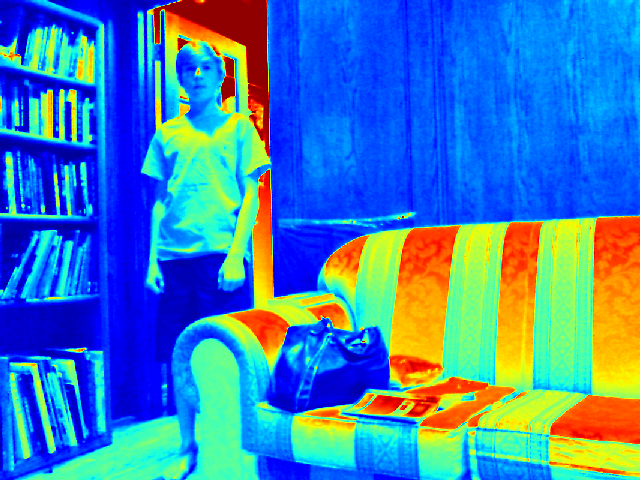
\includegraphics[width=0.45\textwidth]{images/l.png} &
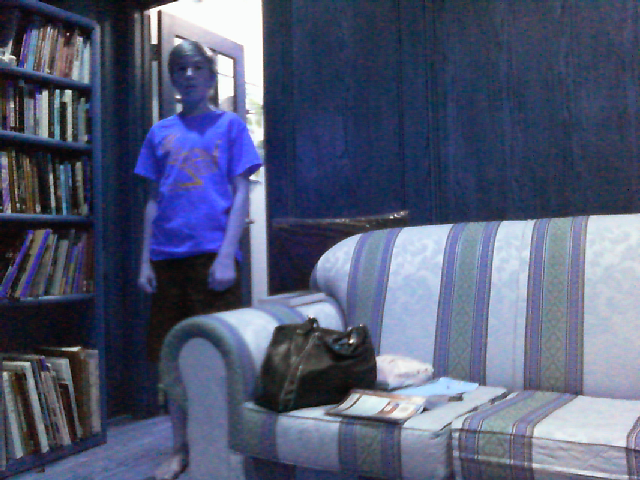
\includegraphics[width=0.45\textwidth]{images/r.png} 
\end{tabular}
\end{center}

\end{frame}
% ................................................


% ................................................
\begin{frame}
\frametitle{Workflow 3: Find distances between images}
This image shows the magnitude of one pixel strips from the images above. Blue is the left image, red is the right image.
\begin{center}
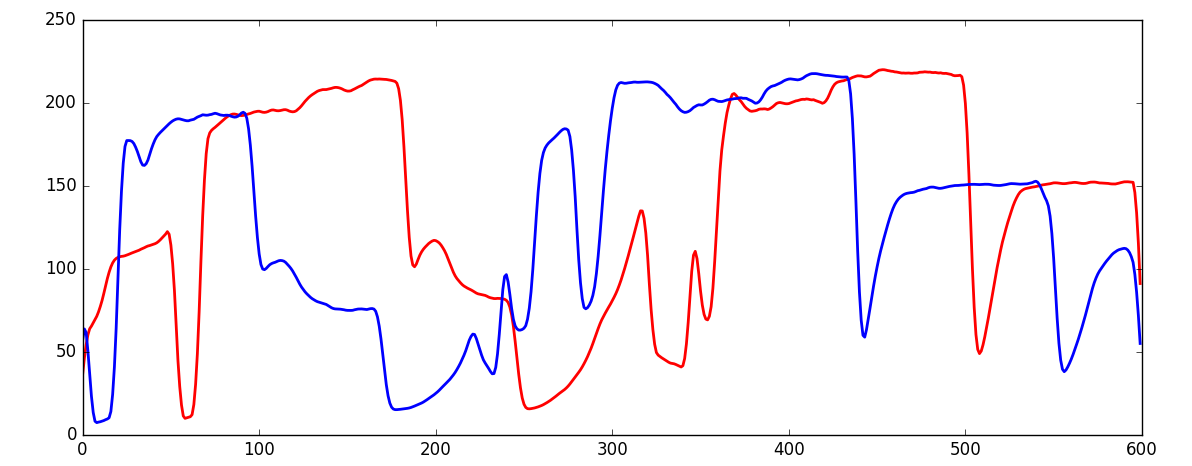
\includegraphics[width=1\textwidth]{images/strips.png} \\[10pt]
\end{center}
The program calculates the pixel distance from the feature on the blue line to the red line, and adds it to the disparity matrix.
\end{frame}
% ................................................


% ................................................
\begin{frame}
\frametitle{Workflow 4: Apply edge preserving median filter (1)}

The disparity maps produced by this technique can be noisy, and we apply filtering in order to reduce the noise.\\[10pt]
%
A median filter works by applying a particular type of edge preserving averaging to pixels. Median filtering is quite simple, requiring two steps per output location:
\begin{enumerate}
\item sort the samples in the input window by magnitude
\item take the median sample value as the output value
\end{enumerate}

We illustrate the application of a 3x3 median filter to random image data on the next slide.

\end{frame}
% ................................................


% ................................................
\begin{frame}
\frametitle{Workflow 4: Apply edge preserving median filter (2)}

\fontsize{8.5}{8.5}\selectfont

\vspace*{-10pt}
\begin{equation*}
\begin{aligned}
&\texttt{4x4 section of representative input image data}\\
& \hspace{20pt} \begin{bmatrix}
2 & 0 & 3 & 5 \\
1 & 4 & 2 & 7 \\
3 & 1 & 0 & 3 \\
6 & 8 & 4 & 2 \\ 
\end{bmatrix} \\[5pt]
%
& \texttt{Application of 3x3 median filter to the $(2,2)$ interior filter location}\\
& \hspace{20pt} \begin{bmatrix}
\mathbf{2} & \mathbf{0} & \mathbf{3} & 5 \\
\mathbf{1} & \mathbf{4} & \mathbf{2} & 7 \\
\mathbf{3} & \mathbf{1} & \mathbf{0} & 3 \\
6 & 8 & 4 & 2 \\ 
\end{bmatrix} 
\rightarrow (2, 0, 3, 1, 4, 2, 3, 1, 0) \rightarrow (0, 0, 1, 1, 2, 2, 3, 3, 4) \rightarrow (2) \\[5pt]
%
& \texttt{Application of 3x3 median filter to the $(3,3)$ interior filter location}\\
& \hspace{20pt} \begin{bmatrix}
2 & 0 & 3 & 5 \\
1 & \mathbf{4} & \mathbf{2} & \mathbf{7} \\
3 & \mathbf{1} & \mathbf{0} & \mathbf{3} \\
6 & \mathbf{8} & \mathbf{4} & \mathbf{2} \\ 
\end{bmatrix} 
\rightarrow (4, 2, 7, 1, 0, 3, 8, 4, 2) \rightarrow (0, 1, 2, 2, 3, 4, 4, 7, 8) \rightarrow (3) \\[5pt]
%
& \texttt{Output 3x3 median filtered data, with edge locations zeroed}\\
& \hspace{20pt} \begin{bmatrix}
0 & 0 & 0 & 0 \\
0 & 2 & 3 & 0 \\
0 & 3 & 3 & 0 \\
0 & 0 & 0 & 0 \\ 
\end{bmatrix}
\end{aligned}
\end{equation*}

\end{frame}
% ................................................


% ................................................
\begin{frame}
\frametitle{Workflow 4: Apply edge preserving median filter (3)}

\vspace*{15pt}
Before/after example of application of a 11x11 median filter applied to a disparity map. The colors correlate with distance: cool colors (blue) are far away, and hot colors (red) are close. \\[10pt]
%
The noise reducing effects of the median filter are evident.

\vspace*{-5pt}
\begin{center}
\begin{tabular}{cc}
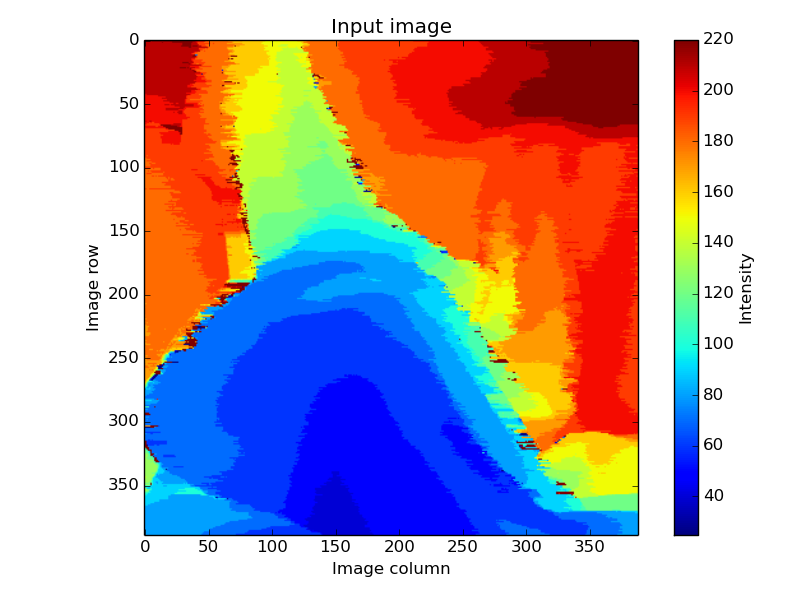
\includegraphics[width=0.49\textwidth, trim=60 10 25 10, clip]{images/median1.png} &
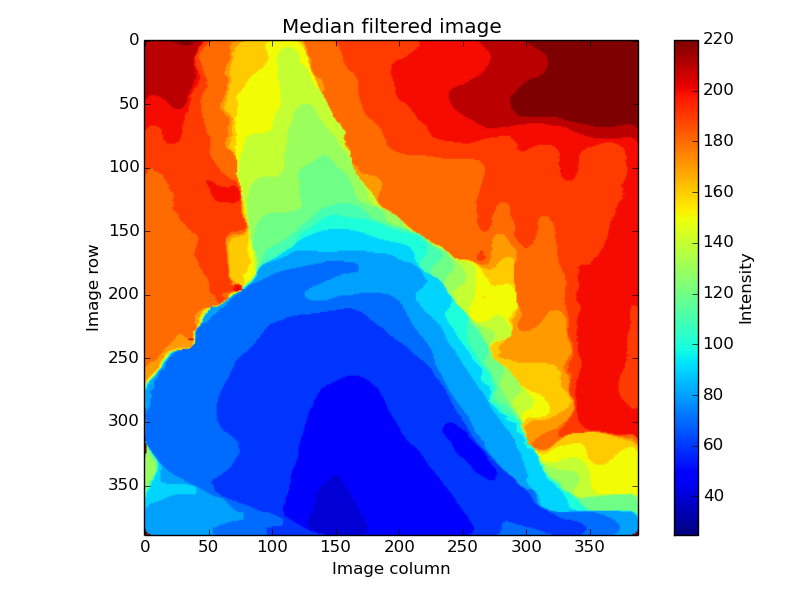
\includegraphics[width=0.49\textwidth, trim=60 10 25 10, clip]{images/median2.png}
\end{tabular}
\end{center}

\end{frame}
% ................................................


% ................................................
\begin{frame}
\frametitle{Workflow 5: Return the final disparity map}

\vspace*{10pt}
The output disparity map has values that do not show distance. To turn these values into distance, the program triangulates using the distance between cameras.\\[10pt]
%
Here are the raw disparity map (left) and the 11x11 median filtered disparity map (right).

\begin{center}
\setlength\tabcolsep{0.01\textwidth}
\begin{tabular}{cc}
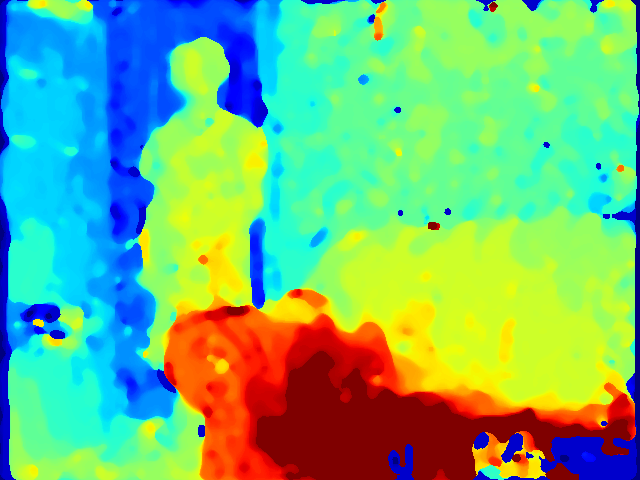
\includegraphics[width=0.45\textwidth]{images/res.png} &
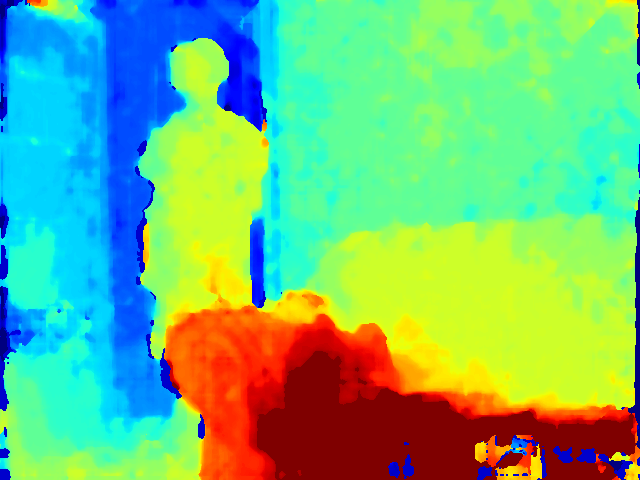
\includegraphics[width=0.45\textwidth]{images/nomedres.png} \\
\end{tabular}
\end{center}

\end{frame}
% ................................................


% ................................................
\begin{frame}
\frametitle{Conclusion}

Disparity maps can be used for many things: traffic control, autonomous cars, and even 3D models. However, the main interest of stereo vision is just how cool it is. \\[10pt]
%
Using stereo vision, computers can tell how far away objects are, and detect obstacles. Stereo vision can make vehicles, drones, and toys smart and sense objects better.\\[10pt]
%
I thought that stereo vision would be much easier than it was, but I am glad that it was hard, because I learned a lot and had a lot of fun.
\end{frame}
% ................................................


\end{document}